% \documentclass{article}
% \usepackage[utf8]{inputenc}
\documentclass{assignment format}
\usepackage{assignment}
\usepackage{bm}
\setcounter{section}{-1}
\setcounter{subsection}{-1}
\usepackage{kotex}

\usepackage{amsmath, amsthm, amssymb}
\usepackage{enumerate}
\usepackage{enumitem}
\usepackage{kotex}
\usepackage{amsfonts}
\usepackage[dvipsnames]{xcolor}
\usepackage{enumitem}
\usepackage{url}
\usepackage{graphicx}
\usepackage{float} 
\usepackage{physics}
\usepackage{bbm}
\usepackage{caption}
\usepackage{minted}
\usepackage{tcolorbox} % Optional: For better code highlighting box style
\usepackage{todonotes}
\usepackage{relsize}
\usepackage{float}
\usepackage{blindtext}
\usepackage{multicol}
\usepackage{xcolor} % to access the named colour LightGray
\definecolor{LightGray}{gray}{0.9}
\newcommand{\note}[4][]{\todo[author=#2,color=#3,size=\scriptsize,fancyline,caption={},#1]{#4}} % default note settings, used by macros below.
\newcommand{\mrinmaya}[2][]{\note[#1]{mrinmaya}{blue!40}{#2}}

\usepackage[colorlinks=true]{hyperref}

\DeclareMathOperator*{\argmax}{arg\,max}

\newenvironment{answer}{
    {\bf Answer:} \begingroup\color{red}
}{\endgroup}%

\begin{document}

\makeheader{\textbf{Due on} Thursday Oct. 10, 2024 \\ by \textbf{23:59 pm}}{Assignment 2}
\begin{center}
%%%%%YOUR NAME HERE%%%%%

\fbox{%
  \parbox{\textwidth}{
  \begin{center}
\large\textbf{Honor Pledge for Graded Assignments}
\\
\\ 
   \large{ “I, YOUR NAME HERE , affirm that I have not given or received any unauthorized help on this assignment, and that this work is my own.”}
    \end{center}
}%
}
\end{center}
\def\showanswers{1}

\section{Instructions (2pts)}
\begin{itemize}
% \item Total score cannot exceed 100 points. For example, if you score 95 points from non-bonus questions and 10 points are added from bonus questions, your score will be 100 points, not 105 points.
% \item You can download the skeleton code file \href{https://raw.githubusercontent.com/yc-song/gsds-nlp-assignment-1/main/a1.zip}{HERE} 
% \item You can download the TeX file \href{https://raw.githubusercontent.com/yc-song/gsds-nlp-assignment-1/main/a1(tex).zip}{HERE} 
\item Skeleton codes for problem 1 and 2 are at the directory \texttt{/skipgram} and \texttt{/sentimentAnalysis} each. 
\item Run the \texttt{bash collect\_submission.sh} script to produce your 2024\_abcde\_coding.zip file. Please make sure to modify collect\_sumbssion.sh file before running this command. (\textbf{abcde} stands for your student id)
\item Modify this tex file into \texttt{a2\_2024-abcde\_written.pdf} with your written solutions
\item Upload both \texttt{2024\_abcde\_coding.zip} and \texttt{2024\_abcde\_written.pdf} to etl website. \textbf{(2pts)}\\
\end{itemize}

%%%NOTE FOR MYSELF%%%


% 40000 ITERATION -> 20000
% list up python files to submit
% dataset 변경

\section{Understanding Skip-Gram (48pts)}

\subsection{Softmax Loss Function}
Word representation by \textbf{Word2vec} is theoretically supported by  \textit{distributional hypothesis}\footnote{The hypothesis that words that occur in similar contexts have similar meanings.} In the example below, a `center' word \textit{banking} is surrounded by `outside' words \textit{turning, into, crises}, and \textit{as} when the context window length is 2.

\begin{figure}[h]
    \centering
    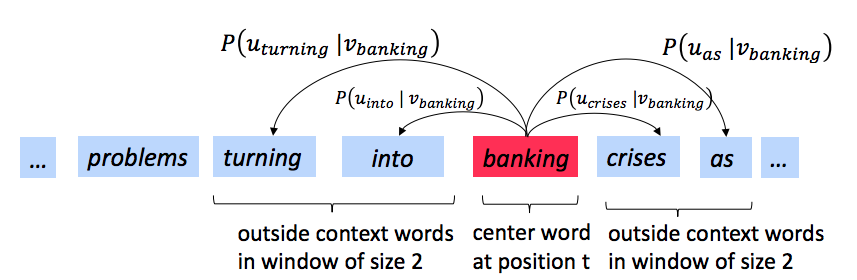
\includegraphics[width=0.6\textwidth]{word2vec.png}
    \caption{The skip-gram prediction model with window size 2}
    \label{fig:word2vec}
\end{figure}
The objective of training Skip-gram is to learn the conditioned probability distribution of outside word {O} given center word \textit{C}, $P(O=o|C=c)$. (i.e. the probability of the word o is an 'outside' word for word c)
The probability can be obtained by taking the softmax function over the inner product of word vectors as below:
\begin{equation}
 P(O=o \mid C=c) = \frac{\exp(\bm u_{o}^\top \bm v_c)}{\sum_{w \in \text{Vocab}} \exp(\bm u_{w}^\top \bm v_c)}
 \label{word2vec_condprob}
\end{equation}
where $u_o$ is the 'outside vector' representing outside word \textit{o}, and $v_c$ is the 'center vector' representing center word c. Be aware that outside and center vector representations of the same word are defined differently.

For the whole vocabulary, we can store outside vector $u_w$ and center vector $v_w$ in two matrices, $U$ and $V$ by columns. That is, the columns of $U$ are all the outside vectors $u_w$ and the columns of $V$ are all the center vectors $v_w$ for every $w \in Vocabulary$


% The true distribution $y$ is a one-hot vector with a 1 for the true outside word o, and 0 everywhere else. The predicted distribution $\hat{y}$ is the probability distribution $P(O|C=c)$ given by Skip-gram model in equation (\ref{word2vec_condprob}).

The loss for a single pair of words $c$ and $o$ is defined as:


\begin{equation}
 J_{\text{naive-softmax}}(\bm v_c, o, \bm U)=-\log P(O=o|C=c)= -\log\frac{\exp(u_{o}^\top v_c)}{\sum_{w \in \text{Vocab}} \exp( u_{w}^\top v_c)}=-u_o^T v_c+\log\sum_{w\in vocab}\exp(u_w^Tv_c)
\label{loss}
\end{equation}


To learn the correct center and outside vector by gradient descent, we need to compute the partial derivative of the outside and center word vectors. Partial derivative of $J_{\text{naive-softmax}}$ with respect to $v_c$ can be obtained as following:
\begin{equation}
\frac{\partial J}{\partial v_c}= -u_o^T+\frac{\sum_{i\in vocab} u_i^T\exp(u_i^Tv_c)}{\sum_{w\in vocab}\exp(u_w^Tv_c)}\\
=-u_o^T+\sum_{i\in vocab}P(O=i|C=c)u_i^T\\= -u_o^T+\sum_{w \in vocab}\hat{y}_wu_w^T\\
= -\mathbf{y}^TU^T+\hat{\mathbf{y}}^TU^T
\label{partial v_c}
\end{equation}where $\mathbf{y}$ is the one-hot vector which has 1 at the index of true outside word $o$ ($y_o=1$ and 0 for all other $i!=o$, $y_i=0$), and 0 everywhere else while $\hat{\mathbf{y}}$ stands for $P(O|C=c)$, a prediction made by Skip-gram model in equation (\ref{word2vec_condprob}).
\begin{enumerate}[label=(\alph*)]
	\item When is the gradient (\ref{partial v_c}) is zero? \textbf{(2pts)}
 %%%%%ANSWER FOR 1.1a%%%%%%
    \begin{answer}

     
    \end{answer}
    \item  If we update $v_c$ with this gradient, toward which vector is $v_c$ getting pulled to?  \textbf{(4pts)}
    \begin{itemize}
    \item \textbf{HINT}: The loss for a single pair of words $c$ and $o$ can be thought of as the cross-entropy between the true distribution \textbf{$y$} and the predicted distribution \textbf{$\hat{y}$} for a particular center word c and outside word o.
\begin{equation} 
\bm J_{\text{naive-softmax}}(\bm v_c, o, \bm U) = -\log P(O=o| C=c) =\\-\sum_{w \in vocab}y_w\log(\hat{y}_w)=-\log{\hat{y}_o}.
\label{naive-softmax}
\end{equation}

\end{itemize}
 %%%%%ANSWER FOR 1.1b%%%%%%
  \begin{answer}
 
    \end{answer}  
    \item Derive the partial derivatives of $J_{\text{naive-softmax}}$ with respect to the outside word vector matrix, $U$.
    \begin{itemize} 
\item \textbf{Note 1}: To get full credit, please write your answer in the form of $v_c, \mathbf{y}$, and $\hat{\mathbf{y}}$ and write the whole computation process. That is, the correct answer does not refer to other vectors but $v_c, \mathbf{y}$, and $\hat{\mathbf{y}}$. 
\item \textbf{Note 2}: Be careful about the dimensions of arrays and matrices. The final answer should have the same shape as U. (i.e. (vector length) $\times$ (vocabulary size)) 
\item\textbf{HINT}: Start from outside word vector $u_w$, which is the column vector of $U$. Then, dividing into two cases may help: when $w=o$ and $w \neq o$ \textbf{(8pts)}
\end{itemize}
%%%%%ANSWER FOR 1.1c%%%%%%
\begin{answer}

    \end{answer}
\end{enumerate}


\subsection{Negative Sampling Loss}
Now we shall consider the Negative Sampling loss, which is an alternative to the Naive Softmax loss.  Assume that $K$ negative samples (words) are randomly drawn from the vocabulary. For simplicity of notation we shall refer to them as $w_1, w_2, \dots, w_K$, and their outside vectors as $\bm u_{w_1}, \bm u_{w_2}, \dots, \bm u_{w_K}$. 
For a center word $c$ and an outside word $o$, the negative sampling loss function is given by:
\begin{equation}
\bm J_{\text{neg-sample}}(\bm v_c, o, \bm U) = -\log(\sigma(\bm u_o^\top \bm v_c)) - \sum_{s=1}^K \log(\sigma(-\bm u_{w_s}^\top \bm v_c))
\label{negsample}
\end{equation}
for a sample $w_1, \ldots w_K$, where $\sigma(\cdot)$ is the sigmoid function.
\begin{enumerate}[label=(\alph*)]
\item Compare the computational complexity of negative sampling with that of the softmax loss function presented in section 1.1. State the reason why negative sampling is computationally more efficient. \textbf{(4pts)}

%%%%%ANSWER FOR 1.2 a%%%%%%
\begin{answer}

    \end{answer}
\item Compute the partial derivatives of $\bm J_{\text{neg-sample}}$ with respect to $\bm v_c$, $\bm u_o$, and the $s^{th}$ negative sample $\bm u_{w_s}$. Please write your answers in terms of the vectors $\bm v_c$, $\bm u_o$, and $\bm u_{w_s}$, where $s \in [1, K]$.
 (within five lines)
\textbf{(8pts)}
%%%%%ANSWER FOR 1.2 b%%%%%%
\begin{answer}
    \end{answer}
\end{enumerate}
\subsection{Coding}
In this part, you will implement the Skip-Gram model and train word vectors with stochastic gradient descent (SGD). Before you begin, first run the following commands within the assignment directory in order to create the appropriate conda virtual environment. This guarantees that you have all the necessary packages to complete the assignment. You will be asked to implement the math functions above using the Numpy package at the root directory. 

\newline \newline
\bold{conda env create -f env.yml} \\
\bold{conda activate a2}
\newline \newline
Once you are done with the assignment you can deactivate this environment by running:
\newline \newline
\bold{conda deactivate}
\newline \newline
For each of the methods you need to implement, we included approximately how many lines of code our solution has in the code comments. These numbers are included to guide you. You don't have to stick to them, you can write shorter or longer code as you wish. If you think your implementation is significantly longer than ours, it is a signal that there are some \texttt{numpy} methods you could utilize to make your code both shorter and faster. \texttt{for} loops in Python take a long time to complete when used over large arrays, so we expect you to utilize \texttt{numpy} methods. The sanity checking function is provided to check if your code works well.
\newline
To run the code command below, please move your directory to \texttt{/skipgram}.
\begin{enumerate}[label=(\alph*)]
    \item We will start by implementing a sampling method in \texttt{utils/treebank.py}. 
        \begin{enumerate}[label=(\roman*)]
            \item Implement the \texttt{sampleTokenIdx} method which first determines sampling frequency per token by reweighting the token frequency and samples a token according to the frequency. \textbf{(4pts)}
            $$\text{index} = \argmax(X), X = (X_1, · · · , X_k)$$
            $$X \sim Multinomial_k(1; p_1, p_2, ..., p_k)) \text{ where } p_i = \frac{(\text{Count}_{w_i})^{0.75}}{\Sigma_{j=1}^{k}{(\text{Count}_{w_j})^{0.75}}}$$
            For more explanation on multinomial distribution, please refer to this \href{http://faculty.washington.edu/yenchic/20A_stat512/Lec7_Multinomial.pdf}{reference}. 
        \end{enumerate}
    \item Now we will implement methods in \texttt{word2vec.py}. You can test a particular method by running \texttt{python word2vec.py m} where \texttt{m} is the method you would like to test. For example, you can test the naiveSoftmaxLossAndGradient method by running \texttt{python word2vec.py naiveSoftmaxLossAndGradient}. (Copy and paste it to your terminal)
        \begin{enumerate}[label=(\roman*)]
        \item Implement the softmax loss and gradient in the \texttt{naiveSoftmaxLossAndGradient} method. \textbf{(6pts)}
        \item Implement the negative sampling loss and gradient in the \texttt{negSamplingLossAndGradient} method. \textbf{(6pts)}
    \end{enumerate}
    \item When you are done, test your entire implementation by running \texttt{python word2vec.py}. Now we are going to load some real data and train word vectors with everything you just implemented! We are going to use The Recognizing Textual Entailment (RTE) dataset to train word vectors. (You can check out the raw datasets in the directory \texttt{./skipgram/utils/datasets/RTE}. There is no additional code to write for this part; just run \texttt{python run.py}.

    (\textbf{Note}: The training process may take a long time depending on the efficiency of your implementation and the computing power of your machine. Please start your homework as soon as possible!)

    After 20,000 iterations, the script will finish and visualization for your word vectors will appear. It will also be saved as \texttt{word\_vectors.png} in your project directory. \textbf{Include the plot below} \textbf{(6pts)}
%%%%%ANSWER FOR 1.3 b%%%%%%
    
    \begin{answer}

    \end{answer}
\end{enumerate}
\section{Sentiment Analysis using Neural Networks (50pts)}

In class, we learned sequence representation and how language models are developed for different tasks. In this assignment, we will implement two neural network models for sentiment analysis task using IMDB dataset. Sentiment analysis in Natural Language Processing (NLP) is a task that involves classifying sentences or text into different categories based on the sentiment expressed. It aims to determine whether the sentiment of the text is positive, or negative. This analysis helps in understanding the overall opinion or emotion conveyed by the text.\\
For this question, please update the given jupyter notebook file in /sentimentAnalysis and submit it along with your answer to this latex file. Please note that this assignment is built and tested under Google Colaboratory. If you work on a local machine, you need to handle version issue on your own. 
\subsection{Multilayer Perceptron (MLP) (30 pts)}
In this question, we are going to implement a simple Multilayer Perceptron (MLP) model to classify IMDB dataset. MLP is the classical type of neural network, and they are comprised of one or more layers of neurons. Data is fed to the input layer, there may be one or more hidden layers providing levels of abstraction, and predictions will be made on the output layer. Please refer to the jupyter notebook for detailed description.
\subsection{Convolutional Neural Network (CNN) (20 pts)}
Next, we will perform sentimental analysis on the same dataset with Convolutional Neural Network (CNN). In a CNN, text is organised into a matrix, with each row representing a word embedding. The CNN’s convolutional layer scans the text like it would an image, breaks it down into features, and judges whether each feature matches the relevant label or not. Implement a CNN model following the instruction in jupyter notebook.

\end{document}
